\section*{ Introduction}

\ifthenelse{\boolean{isXavier}}{%if is Xavier
%%% Slide for Xavier %%%
\begin{frame}[c,noframenumbering]
   \frametitle{Who am I?}

   \begin{columns}[T]
     \begin{column}{0.65\linewidth}
         \textbf{Xavier Corbillon}

         First year PhD student at Telecom Bretagne
      \end{column}
      \begin{column}{0.35\linewidth}
         
\includegraphics[scale=0.25]{plots/pictures/Xavier/idCard.eps}
      \end{column}
   \end{columns}

   \vspace{-0.5cm}
   % 
\includegraphics[scale=0.25]{plots/pictures/Xavier/ritelogo.jpg}
   %
   % 
\includegraphics[scale=0.125]{plots/pictures/Xavier/neo-telecoms.jpg}
   % \hspace{2cm}
   % 
\includegraphics[scale=0.5]{plots/pictures/Xavier/ABB.jpg}

   \only<1-5>{
   \tikzsetnextfilename{timeline}
   \begin{tikzpicture}
      \newlength{\timeLength}
      \setlength{\timeLength}{10cm}

      \pgfdeclareimage[width=0.2\timeLength]{rite}{plots/pictures/Xavier/ritelogo.jpg}
      \pgfdeclareimage[width=0.2\timeLength]{neo}{plots/pictures/Xavier/neo-telecoms.jpg}
      \pgfdeclareimage[width=0.2\timeLength]{abb}{plots/pictures/Xavier/ABB.jpg}

      %timeline
      \draw[->] (0,0) -- ++(\timeLength+1cm, 0) node[below] {t};

      \coordinate (2010) at (0.1\timeLength,0);
      \coordinate (2011) at (0.1\timeLength+0.15\timeLength,0);
      \coordinate (2012) at (0.1\timeLength+0.30\timeLength,0);
      \coordinate (2013) at (0.1\timeLength+0.45\timeLength,0);
      \coordinate (2014) at (0.1\timeLength+0.60\timeLength,0);
      \coordinate (2015) at (0.1\timeLength+0.75\timeLength,0);
      \coordinate (2016) at (0.1\timeLength+0.90\timeLength,0);

      \incBP{1}
      \onslide<+->{
         \node at (0.1\timeLength+0.1\timeLength,1cm) (tb) {
\includegraphics[width=0.12\timeLength, keepaspectratio]{Modele/bretagne_quadri_et_baseline}};
         \draw[beamer@tbgreen, thick] (2010) -- (2012);
         \draw[beamer@tbgreen, thick] (2013) -- (2014);
      }

      \definecolor{whiteblue}{HTML}{729FCF}
      \onslide<+->{
         \node at (0.1\timeLength+0.35\timeLength,1.2cm) (Neo) {\pgfuseimage{neo}};
         \draw[whiteblue, thick] (2012) -- (2013);
      }

      \onslide<+->{
         \node at (0.1\timeLength+0.65\timeLength,1cm) (abb) {\pgfuseimage{abb}};
         \draw[red, thick] (2014) -- (2015);
      }

      \onslide<+->{
         \node at (0.1\timeLength+0.85\timeLength,1cm) (rite) {\pgfuseimage{rite}};
         \draw[beamer@tbgreen, thick] (2015) -- (\timeLength+0.99cm,0);
         \draw[whiteblue, thick, dashed] (2015) -- (2016);
      }

      \foreach \t in {2010, 2011, 2012, 2013, 2014, 2015, 2016}{
         \draw (\t) ++(0, -0.05cm) -- ++(0,0.1cm);
         \node[below] at (\t) {\scriptsize \t};
      }

   \end{tikzpicture}
   }
\end{frame}
}{%then is not Xavier
   \ifthenelse{\boolean{isGwendal}}{ % if Gwendal
   %%% Slide for Gwendal  %%%
   \begin{frame}[c,noframenumbering]
      \frametitle{Who am I?}

      \textbf{Gwendal Simon}

   \end{frame}
   }
   { % is not gwendal

   }
}


\ifthenelse{\boolean{is5G}}{
    %%% Slide 5G  %%
\begin{frame}[c,noframenumbering]
   \frametitle{5G}
   Test
\end{frame}

}{}

%%% Slide  %%%
\newcounter{tmpCounter1}
\newcounter{tmpCounter2}
\newcommand{\boldWhenNeeded}[1]{\only<.-\arabic{tmpCounter1}>{#1} \only<\arabic{tmpCounter2}->{\textbf{#1}}}
\begin{frame}[c]
   \frametitle{Context: 360-Degree Videos}

   \vfill

   \setcounter{tmpCounter2}{\valueBP+6}
   \setcounter{tmpCounter1}{\value{tmpCounter2}-1}
   \begin{columns}[T]
     \begin{column}{0.65\linewidth}
        \begin{itemize}
           \item<+-> \textbf{Applications}:
            \begin{itemize}[<+->]
               \item Gaming
               \item \boldWhenNeeded{Documentaries}
               \item \boldWhenNeeded{Recorded sports and concerts}
               \item \boldWhenNeeded{Adult content}
               \item \boldWhenNeeded{Live event broadcast}
               \item Education and Training
            \end{itemize}
         \end{itemize}
     \end{column}
     \begin{column}{0.35\linewidth}
         %\begin{itemize}[<+->]
         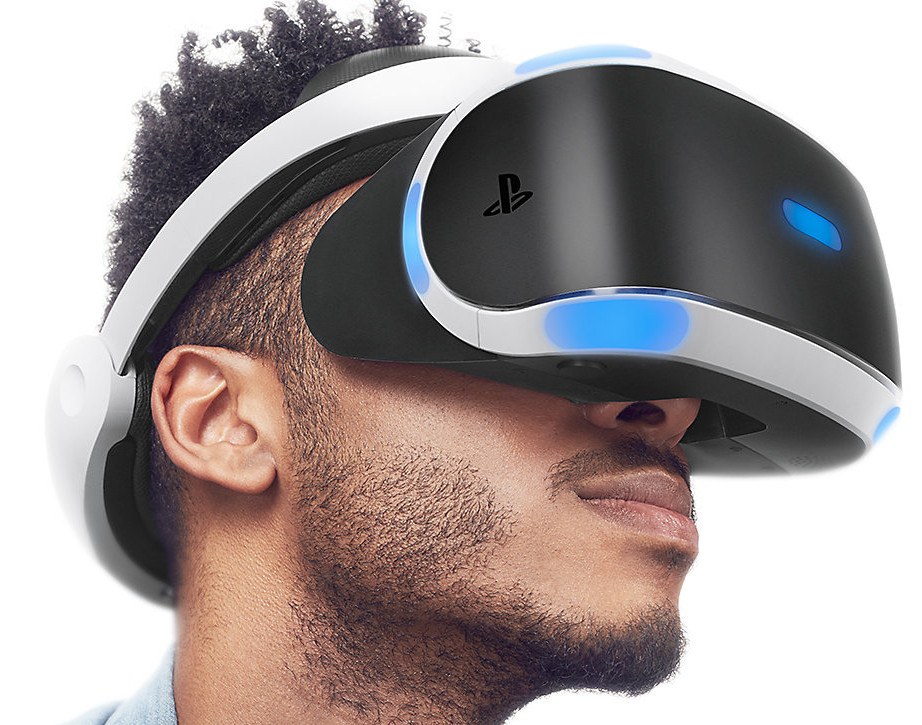
\includegraphics[scale=0.125]{plots/pictures/playstation-vr.jpg}\\
         \vspace{-0.25cm}
         {}%\tiny Source: playstation.com}
         %\end{itemize}
     \end{column}
   \end{columns}

   %\end{itemize}
   %\incBP{1}
   \vfill
   %\vspace{-0.5cm}
   %\href{run:videos/car_equirectangular_4k.mp4}{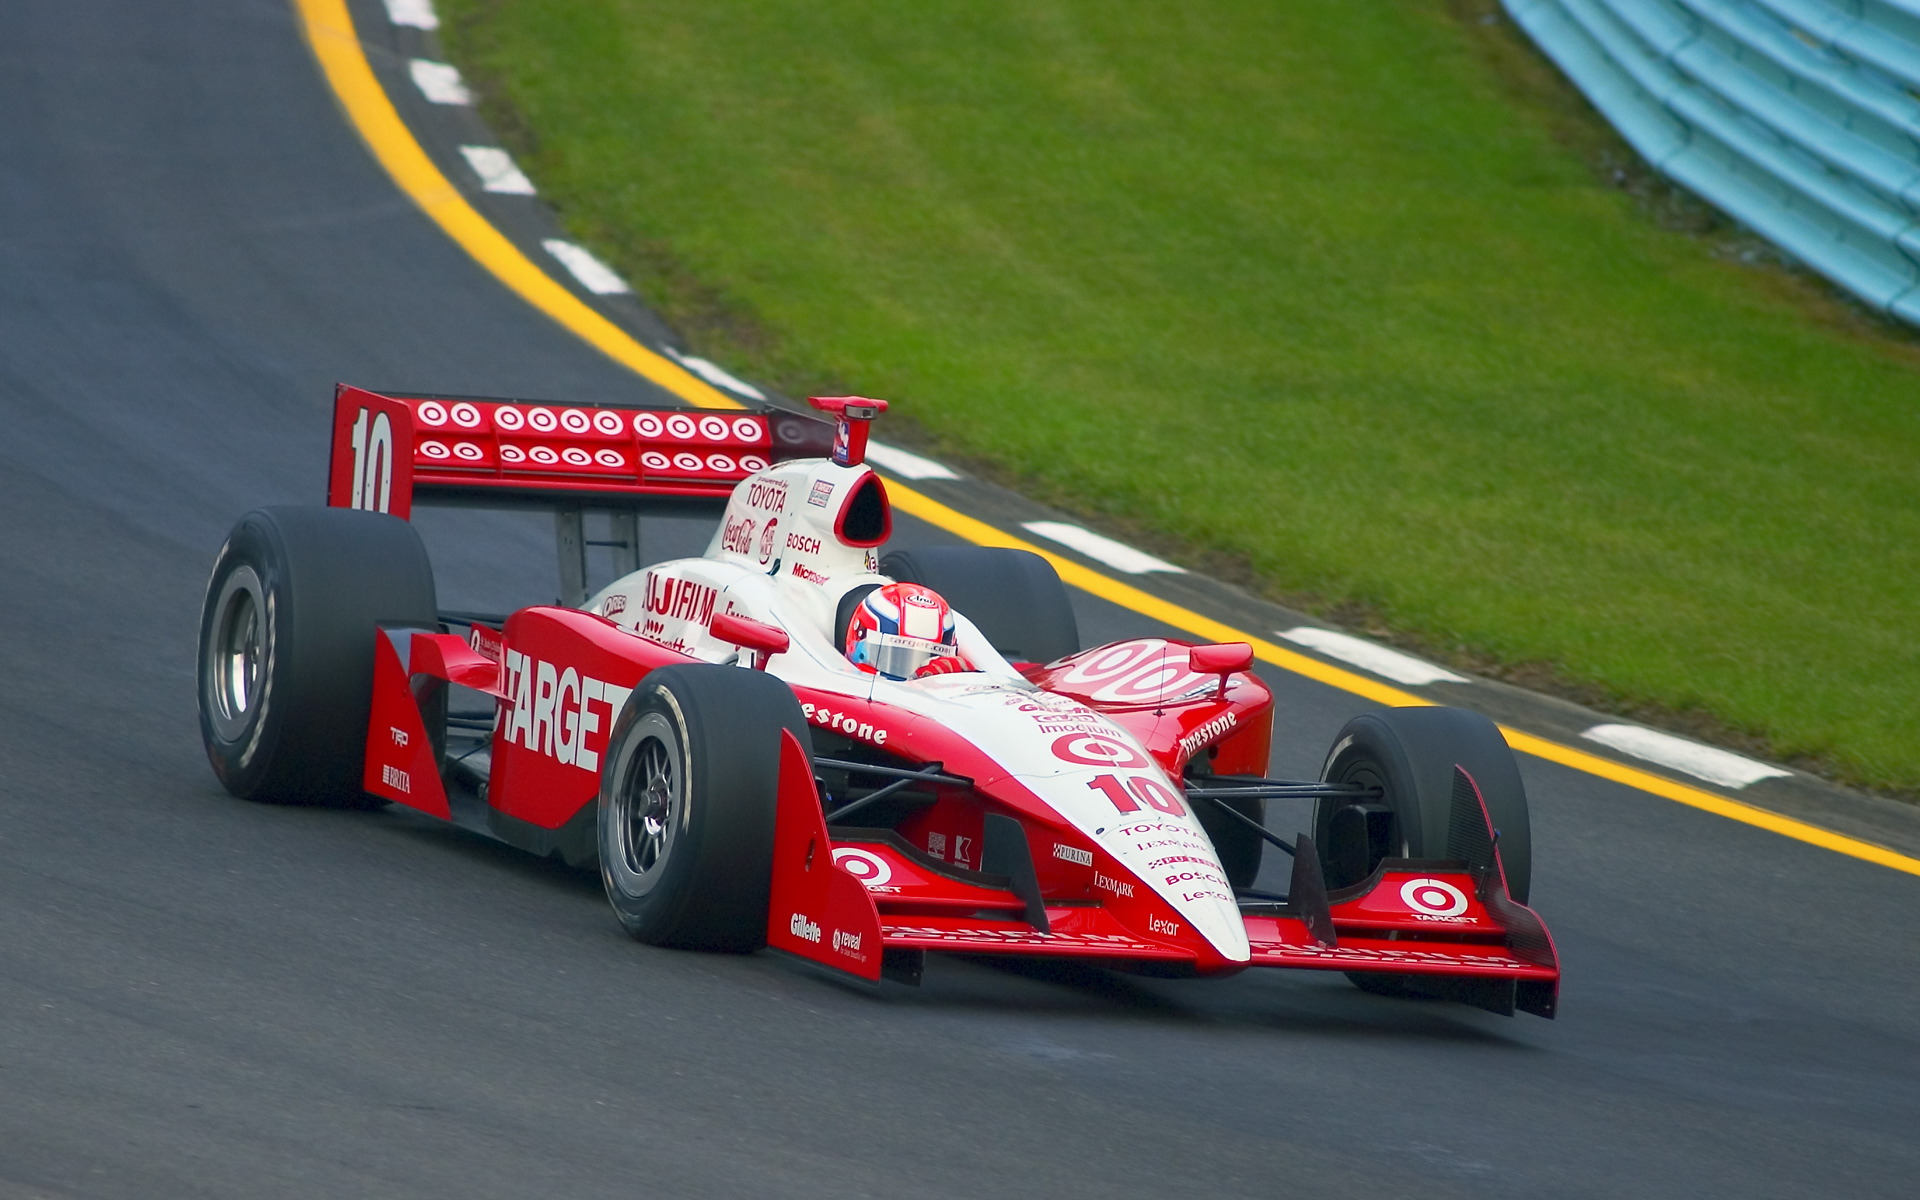
\includegraphics[scale=0.3]{videos/test.jpg}}
   \begin{minipage}[t][4cm][t]{\textwidth}
      \only<+-.(4)>{
         \begin{itemize}[<.->]
            \item Omnidirectional video:
         \end{itemize}
         \begin{columns}[T]
            \begin{column}{0.5\linewidth}
               %\onslide<.-.(3)>{
               \begin{independentCounter}
                  %\decBP{1}
                  \begin{figure}[h]
\centering
\begin{tikzpicture}


\tikzset{
     element/.style={
     	rounded corners,
     	rectangle,
  	 	thick,
  	 	draw=black,
  	 	minimum height=2cm,minimum width=2.5cm
     }
}

\tikzset{
	elementtitle/.style={
		rectangle,
		rounded corners,
		fill=gray!80,
		font=\footnotesize,
		text=white,
		anchor=north
	}
}

\tikzset{
	pics/equirec/.style n args={3}{
		code={
			\draw[fill=gray!30] (-0.0352778*#1, -0.019844*#1) rectangle (0.0352778*#1, 0.019844*#1);
			\draw[draw=none,fill=gray!70] (0.0088194*#2*#1-2*0.0088194*#1, 0.0066147*#3*#1 - 2*0.0066147*#1) rectangle (0.0088194*#2*#1 + 2*0.0088194*#1, 0.0066147*#3*#1 + 2*0.0066147*#1);
			\draw[draw,fill=none] (-0.0352778*#1, -0.019844*#1) rectangle (0.0352778*#1, 0.019844*#1);
			\draw[color=black,fill=black] (0.0088194*#2*#1, 0.0066147*#3*#1) circle (1pt);
		}		
	}
}

\def\convCmPt{0.0352778}
\def\convCmPtRec{0.019844}
\def\convCmPtRecThird{0.0066147}
\def\convCmPtFourth{0.0088194}

\tikzset{cross/.style={cross out, draw,
         minimum size=2*(#1-\pgflinewidth),
         inner sep=0pt, outer sep=0pt}}

\tikzset{
	fov/.pic ={
		\draw[densely dotted, thick, red!70!black] (-0.07,0.10) rectangle (0.37,-0.20);
%		\draw[fill=red] (0.2,-0.05) circle (2pt);
		\draw (0.15,-0.05) node[cross=2pt,red!70!black] {};
	}
}


\tikzset{
	vr/.pic = {
		\draw[rounded corners] (-0.0352778*#1, -0.019844*#1) rectangle (0.0352778*#1, 0.019844*#1);
		\draw[rounded corners, thick] (-0.032*#1, -0.019844*#1) rectangle (0.032*#1, 0.016*#1);
%		\draw(-0.019*#1,0) pic {fov};
%		\draw(0.019*#1,0) pic {fov};
		\node[font=\scriptsize,rectangle,red, draw=red, thick,
					densely dotted, anchor=east, inner sep=2pt,
					yshift=-1pt, xshift=-1pt] at (0,0) {L};
		\node[font=\scriptsize,rectangle,red, draw=red, thick,
					densely dotted, anchor=west, inner sep=2pt,
					yshift=-1pt,xshift=0.5pt] at (0,0) {R};
	}
}
		
\def\ecartElement{20pt}
\def\sizeSphere{11}
\def\ecartObjet{2}
\def\ecartYVersions{16pt}


% capturing system
\node[element] (0,0) (capturing) {};
\node[elementtitle, above=-5pt of capturing] {capturing};
\draw ([xshift=-\sizeSphere - \ecartObjet pt]capturing.east) pic {spherical=\sizeSphere};
\pgfdeclareimage[width=18 pt]{camera}{video-camera-icon-hi.png}
\node at ([xshift=21 pt]capturing.west) (camera1)
    {\pgfbox[right,center]{\pgfuseimage{camera}}};

% the arrow in the capture
\draw[-latex] (camera1.east) to ([xshift=-2*\sizeSphere - 2*\ecartObjet pt]capturing.east);


% ===== server
\node[element,right=\ecartElement of capturing] (server) {};
\node[elementtitle, above=-5pt of server] {\vphantom{pt}server};
\draw ([xshift=\sizeSphere + \ecartObjet pt]server.west) pic {spherical=\sizeSphere};
\draw ([xshift=-\sizeSphere - \ecartObjet pt]server.east) pic {equirec={\sizeSphere}{2}{1}};
\draw ([xshift=-\sizeSphere - \ecartObjet pt, yshift=\ecartYVersions]server.east) pic {equirec={\sizeSphere}{-2}{-1}};
\draw ([xshift=-\sizeSphere - \ecartObjet pt, yshift=-\ecartYVersions]server.east) pic {equirec={\sizeSphere}{0}{0}};

% the three arrows in the server
\draw[-latex] ([xshift=2*\sizeSphere + 2*\ecartObjet pt]server.west) to ([xshift=-2*\sizeSphere - 2*\ecartObjet pt]server.east);
\draw[-latex] ([xshift=2*\sizeSphere + 2*\ecartObjet pt]server.west) to ([xshift=-2*\sizeSphere - 2*\ecartObjet pt, yshift=\ecartYVersions]server.east);
\draw[-latex] ([xshift=2*\sizeSphere + 2*\ecartObjet pt]server.west) to ([xshift=-2*\sizeSphere - 2*\ecartObjet pt, yshift=-\ecartYVersions]server.east);

% between capture and server
\draw[-latex] ([xshift=2pt]capturing.east) to ([xshift=-2pt]server.west);


% ===== client
\node[element,right=\ecartElement of server] (client) {};
\node[elementtitle, above=-5pt of client] {\vphantom{pt}client};
% the equirecntagular
\draw([xshift=\sizeSphere + \ecartObjet pt, yshift=-\ecartYVersions]client.west) pic {equirec={\sizeSphere}{0}{0}};
% the old vr
%\draw ([xshift=-\sizeSphere - \ecartObjet pt]client.east) pic {vr=\sizeSphere};
% the fov
\pic[local bounding box=thisfov] at ([xshift=\sizeSphere + \ecartObjet pt, yshift=-\ecartYVersions]client.west) {fov};
%\node[anchor=west, font=\tiny,red, text width=23pt,align=center]
%		at ([yshift=10pt]client.west) (fovleg) {\ac{FoV} and \ac{FoV} center};
%
%\draw[red] (fovleg) -- (thisfov);

% vr headset
\pgfdeclareimage[width=24 pt]{vrheadset}{vr_icon.png}
\node at ([xshift=-28 pt]client.east) (headset)
    {\pgfbox[left,center]{\pgfuseimage{vrheadset}}};

% old vr
%

% the arrow in the client
\draw[-latex] 
%	([xshift=2*\sizeSphere + 2*\ecartObjet pt, yshift=-\ecartYVersions]client.west) to 
	(thisfov.60) to
		([xshift=-2*\sizeSphere - 2*\ecartObjet pt]client.east);


% between server and client
\draw[-latex] ([xshift=2pt, yshift=-\ecartYVersions]server.east) to ([xshift=-2pt, yshift=-\ecartYVersions]client.west);


\end{tikzpicture}
\caption{\ac{FoV}-adaptive 360-degree video delivery system: The server
offers video representations for three \acp{QEC}. The dark grey is the part of the video encoded at high quality and the light
gray the low quality. The \ac{FoV} video is the dotted red rectangle, and the \ac{FoV} center is the
cross}
\label{fig:deliverychain}
\end{figure}

               \end{independentCounter}
               %}
            \end{column}
            \begin{column}{0.5\linewidth}
               \only<.>{
                  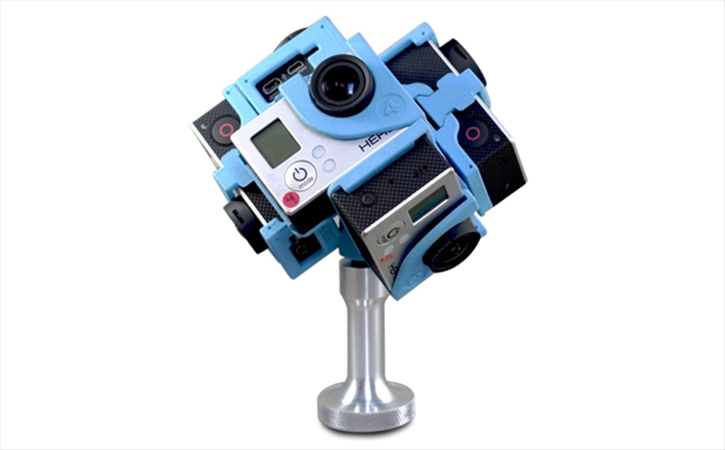
\includegraphics[scale=0.15]{videos/360camera1.png}
                  \includegraphics[scale=0.02]{videos/360camera2.jpg}
                  \setcounter{tmpCounter}{\value{beamerpauses}}
               }
               \only<.(1)>{\hspace{2cm}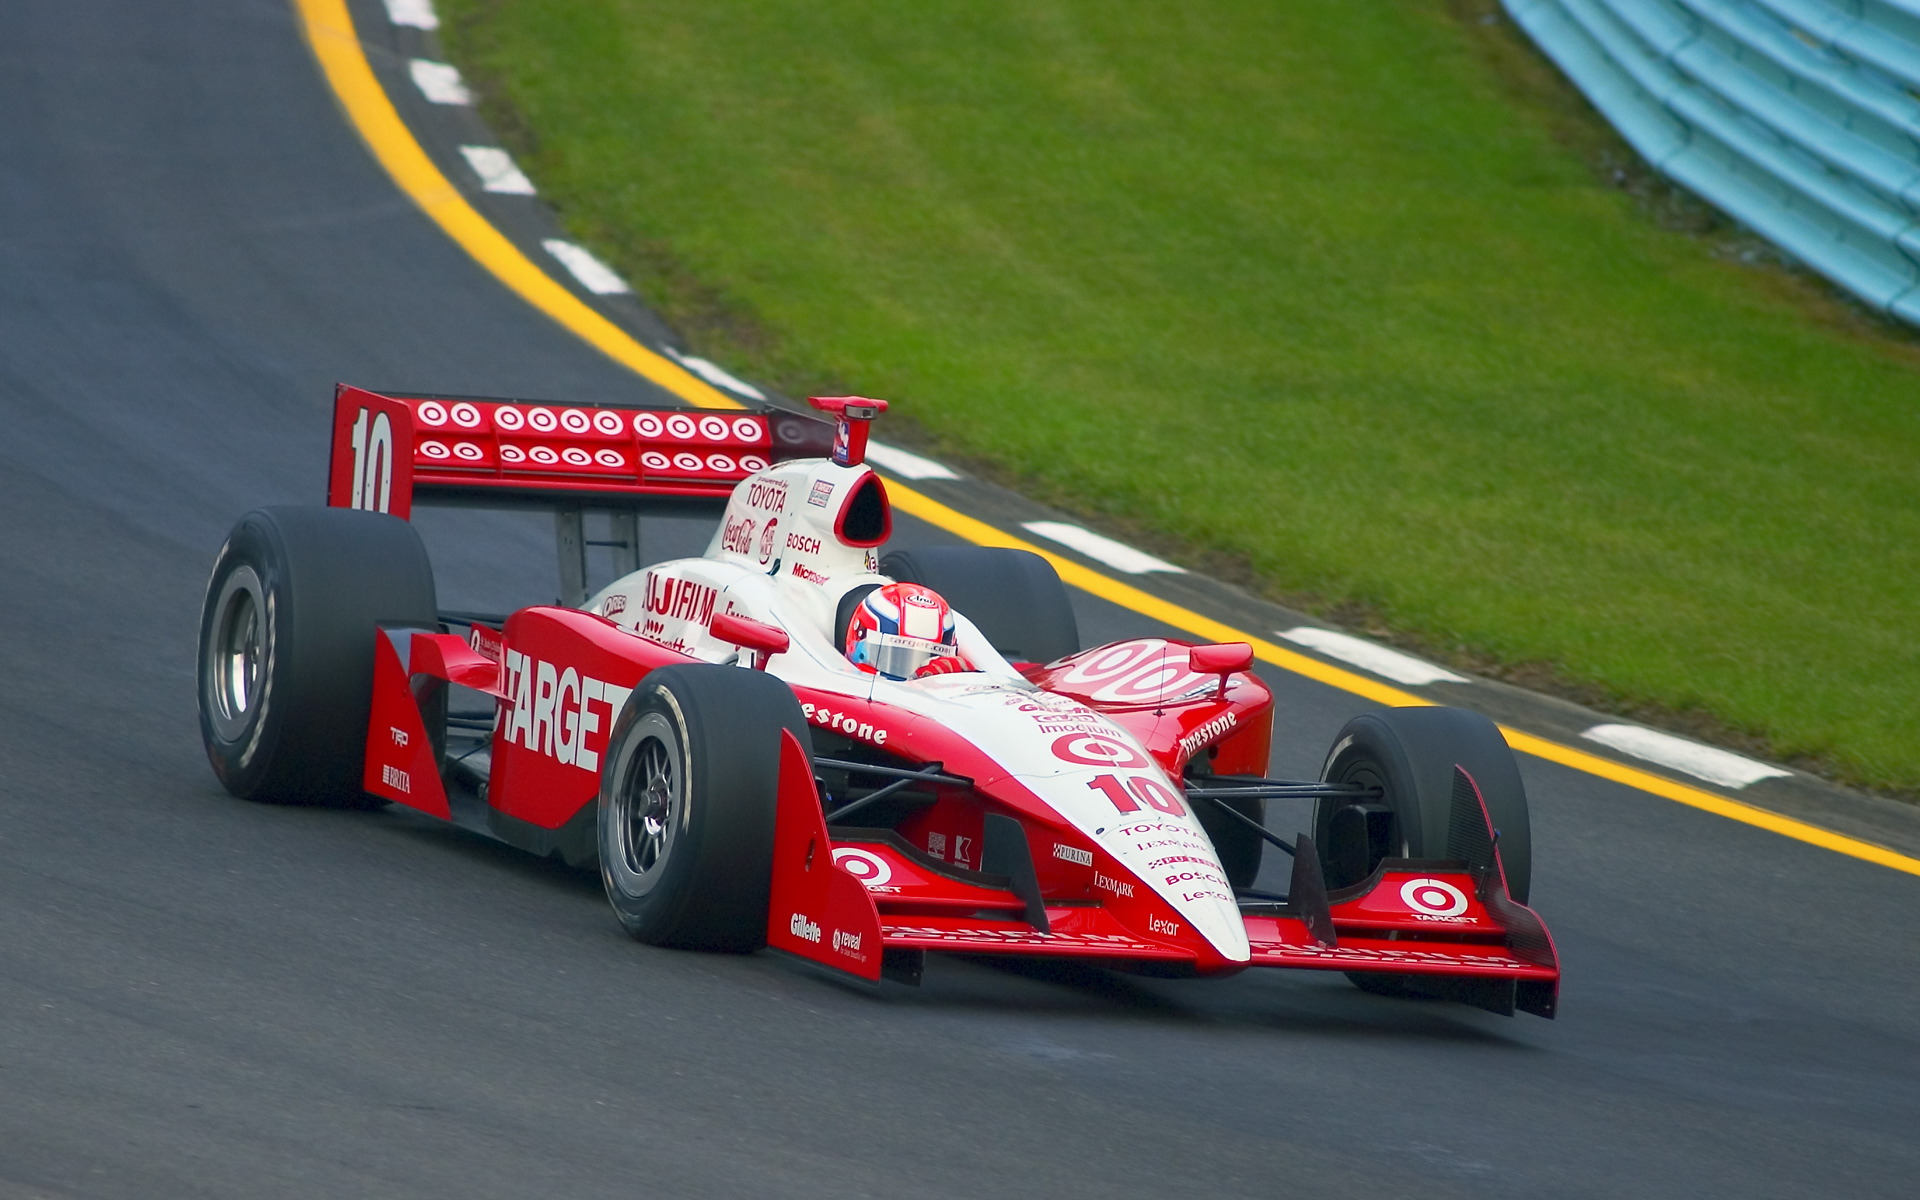
\includegraphics[scale=0.04]{videos/test.png}}
               \only<.(2)>{\hspace{2cm}
\includegraphics[scale=0.065]{videos/fov1.png}}
               \only<.(3)>{\hspace{2cm}
\includegraphics[scale=0.065]{videos/fov2.png}}
            \end{column}
         \end{columns}
         % \onslide<.>{
         % \vspace{-0.75cm}
         % {
         %    \tiny
         %    %\url{http://360cameraonline.com/wp-content/uploads/2015/01/gopro_360camera.png}
         % }\\
         %
         % {\vspace{-0.75cm}
         %    %\tiny \url{https://mms.businesswire.com/media/20151221005321/en/501689/5/PANONO_BACK_PRESS_RGB.jpg}
         % }
         %}
      }
      \incBP{2}
      \only<+->{
         \vfill
         \begin{itemize}[<+->]
            \item \textbf{Problem}: 4K stereo videos + 100\,fps $\Rightarrow$ $>$  100\,Mbps
         \end{itemize}
         \vspace{2cm}
      }
    \end{minipage}
    \vfill
\end{frame}

\begin{frame}[c]
   \frametitle{How to deliver videos today?}

   \begin{itemize}
     \item \textbf{Main technology}: \acl{HAS}
     \begin{itemize}
        \setbeamercovered{transparent}
        \item MPEG-DASH\uncover<+>{, Apple HLS, Adobe HDS, MSS}
        \setbeamercovered{invisible}
     \end{itemize}
   \end{itemize}
   \begin{minipage}[t][7cm][t]{\textwidth}
   \only<+>{
   \raggedright
   \textbf{Concept}:\\
   \centering
   \only<2>{}
\tikzsetnextfilename{dash}
\begin{tikzpicture}

\tikzset{
     element/.style={
     	rounded corners,
     	rectangle,
  	 	thick,
  	 	draw=black,
  	 	minimum height=2cm,minimum width=2.5cm
     }
}

\tikzset{
	elementtitle/.style={
		rectangle,
		rounded corners,
		fill=gray!80,
		font=\footnotesize,
		text=white,
		anchor=north
	}
}

% this is the equirectangular with QEC and qualities
\tikzset{
	pics/equirec/.style n args={3}{
	% the first parameter is the size
	% the second parameter is the x coordinate of the QEC
	% the third parameter is the y coordinate of the QEC
		code={
			\draw[fill=gray!30] (-0.0352778*#1, -0.019844*#1) rectangle (0.0352778*#1, 0.019844*#1);
			%\draw[draw=none,fill=gray!70] (0.0088194*#2*#1-2*0.0088194*#1, 0.0066147*#3*#1 - 2*0.0066147*#1) rectangle (0.0088194*#2*#1 + 2*0.0088194*#1, 0.0066147*#3*#1 + 2*0.0066147*#1);
			\draw[draw,fill=none] (-0.0352778*#1, -0.019844*#1) rectangle (0.0352778*#1, 0.019844*#1);
			%\draw[color=black,fill=black] (0.0088194*#2*#1, 0.0066147*#3*#1) circle (1pt);
		}
	}
}

\tikzset{
	emptyEquirec/.pic={
		\draw[fill=gray!30] (-0.0352778*#1, -0.019844*#1) rectangle (0.0352778*#1, 0.019844*#1);
	}
}

\def\convCmPt{0.0352778}
\def\convCmPtRec{0.019844}
\def\convCmPtRecThird{0.0066147}
\def\convCmPtFourth{0.0088194}

\tikzset{cross/.style={cross out, draw,
         minimum size=2*(#1-\pgflinewidth),
         inner sep=0pt, outer sep=0pt}}

% here is for the FoV
\tikzset{
	pics/fov/.style n args={2}{
		% the first parameter is the size of the screen
		% the second parameter is the x coordinate of the FoV center (0, 1 or 2)
		code = {
			\draw (-0.5*#1, -0.28*#1) rectangle (0.5*#1, 0.28*#1);
			\draw[densely dotted, thick, red!70!black] (-0.45*#1 + #2*#1*0.24, 0.15*#1)
				 rectangle
			 	(-0.4*#1 + #2*#1*0.24 + 0.4*#1, -0.15*#1);
			\draw (-0.4*#1 + #2*#1*0.24 + 0.2*#1, 0.05*#1) node[cross=2pt,red!70!black] {};
	   }
	}
}


\tikzset{
	vr/.pic = {
		\draw[rounded corners] (-0.0352778*#1, -0.019844*#1) rectangle (0.0352778*#1, 0.019844*#1);
		\draw[rounded corners, thick] (-0.032*#1, -0.019844*#1) rectangle (0.032*#1, 0.016*#1);
		\node[font=\scriptsize,rectangle,red, draw=red, thick,
					densely dotted, anchor=east, inner sep=2pt,
					yshift=-1pt, xshift=-1pt] at (0,0) {L};
		\node[font=\scriptsize,rectangle,red, draw=red, thick,
					densely dotted, anchor=west, inner sep=2pt,
					yshift=-1pt,xshift=0.5pt] at (0,0) {R};
	}
}

% this is for three representations at different sizes for a given QEC
\tikzset{
	pics/threerep/.style n args={5}{
	% first parameter is a bool if bw must be written
	% second parameter is the QEC number (0 if not displayed)
	% third parameter is the segment number (0 if not displayed)
	% fourth parameter is the x pos of QEC
	% fifth paramerer is the y pos of QEC
		code={
			\pic[local bounding box=bigA] at (0,0) {equirec={\sizeBig}{#4}{#5}};
			\ifnum#1>0
		    	\node[font=\scriptsize, anchor=east, inner sep=0pt]
		    		at (bigA.west) (legbwhi) {high};
		    \fi
		    \ifnum#3>0
				\node[font=\scriptsize,anchor=south] at (bigA.north) {$s_{#3}$};
			\fi
			\pic[local bounding box=medA] at ([yshift=\ecartMed]bigA.south) {equirec={\sizeMed}{#4}{#5}};
			\ifnum#1>0
				\node[font=\scriptsize,anchor=west, inner sep=0pt]
					at (legbwhi.west |- medA) (legbwme) {\vphantom{g}med};
			\fi
			\pic[local bounding box=lowA] at ([yshift=\ecartLow]medA.south)
				{equirec={\sizeLow}{#4}{#5}};
			%\pic[local bounding box=lowA] at ([yshift=\ecartLow]bigA.south)
			%	{equirec={\sizeLow}{#4}{#5}};
			\ifnum#1>0
				\node[font=\scriptsize, inner sep=0pt, anchor=west]
					at (legbwme.west |- lowA) {\vphantom{g}low};
			\fi
			\ifnum#2>0
				\node[font=\footnotesize,anchor=east] at (legbwhi.south west) {QEC$_#2$};
			\fi
		}
	}
}

% this is for the guy looking at the left
\tikzset{
	leftVR/.pic = {
	% the only parameter is the size
		% first the body
		\draw plot [smooth] coordinates {(0,0)
			(0.05*#1,0.2*#1)
			(0.25*#1,0.2*#1)
			(0.3*#1,0)};
		\draw (0,0) -- (0.3*#1,0);
		% then the head
		\draw[fill=white] (0.15*#1, 0.4*#1) ellipse (0.15*#1 cm and 0.2*#1 cm);
		% then the VR headset
		\draw[rounded corners=0.3*#1, fill=black] (-0.03*#1, 0.55*#1) rectangle
			(0.1*#1, 0.35*#1);
		\begin{scope}
			\clip (0.15*#1, 0.4*#1) ellipse (0.15*#1 cm and 0.2*#1 cm);
			\draw[fill=black] (0.1*#1, 0.5*#1) rectangle (0.3*#1, 0.46*#1);
			\draw plot [smooth] coordinates {(-0.01*#1,0.3*#1)
			 (0.04*#1,0.27*#1)
			 (0.09*#1,0.3*#1)};
		\end{scope}
	}
}

% this is for the guy looking at the right
\tikzset{
	rightVR/.pic = {
	% the only parameter is the size
		% first the body
		\draw plot [smooth] coordinates {(0,0)
			(0.05*#1,0.2*#1)
			(0.25*#1,0.2*#1)
			(0.3*#1,0)};
		\draw (0,0) -- (0.3*#1,0);
		% then the head
		\draw[fill=white] (0.15*#1, 0.4*#1) ellipse (0.15*#1 cm and 0.2*#1 cm);
		% then the VR headset
		\draw[rounded corners=0.3*#1, fill=black] (0.33*#1, 0.55*#1) rectangle
			(0.2*#1, 0.35*#1);
		\begin{scope}
			\clip (0.15*#1, 0.4*#1) ellipse (0.15*#1 cm and 0.2*#1 cm);
			\draw[fill=black] (0.2*#1, 0.5*#1) rectangle (0, 0.46*#1);
			\draw plot [smooth] coordinates {(0.22*#1,0.3*#1)
			 (0.27*#1,0.27*#1)
			 (0.32*#1,0.3*#1)};
		\end{scope}
	}
}

% this is for the guy looking at the front
\tikzset{
	frontVR/.pic = {
	% the only parameter is the size
		% first the body
		\draw plot [smooth] coordinates {(0,0)
			(0.08*#1,0.2*#1)
			(0.42*#1,0.2*#1)
			(0.5*#1,0)};
		\draw (0,0) -- (0.5*#1,0);
		% then the head
		\draw[fill=white] (0.25*#1, 0.4*#1) ellipse (0.15*#1 cm and 0.2*#1 cm);
		\draw plot [smooth] coordinates {(0.18*#1,0.3*#1)
			 (0.25*#1,0.27*#1)
			 (0.32*#1,0.3*#1)};
		% then the VR headset
		\draw[rounded corners=0.5*#1, fill=black] (0.07*#1, 0.55*#1) rectangle
			(0.43*#1, 0.35*#1);
	}
}


\def\sizeBig{11}
\def\sizeMed{9}
\def\ecartMed{-12 pt}
\def\sizeLow{7}
\def\ecartLow{-12 pt}
\def\ecartInterThree{-0.52}


\pic[local bounding box=leftup] at (0,0) {threerep={1}{0}{1}{2}{1}};
% \pic[anchor=east, local bounding box=leftmid] at ($(-0.4,\ecartInterThree)+(leftup.east |- leftup.south)$)
% 	  {threerep={1}{2}{0}{-2}{-1}};
% \pic[anchor=east, local bounding box=leftdown] at ($(-0.4,\ecartInterThree)+(leftmid.east |- leftmid.south)$)
% 	  {threerep={1}{3}{0}{0}{0}};

\pic[local bounding box=centerup] at (1,0) {threerep={0}{0}{2}{2}{1}};
% \pic[anchor=east, local bounding box=centermid] at ($(-0.4,\ecartInterThree)+(centerup.east |- centerup.south)$)
% 	  {threerep={0}{0}{0}{-2}{-1}};
% \pic[anchor=east, local bounding box=centerdown] at ($(-0.4,\ecartInterThree)+(centermid.east |- centermid.south)$)
% 	  {threerep={0}{0}{0}{0}{0}};

\pic[local bounding box=rightup] at (2,0) {threerep={0}{0}{3}{2}{1}};
% \pic[anchor=east, local bounding box=rightmid] at ($(-0.4,\ecartInterThree)+(rightup.east |- rightup.south)$)
% 	  {threerep={0}{0}{0}{-2}{-1}};
% \pic[anchor=east, local bounding box=rightdown] at ($(-0.4,\ecartInterThree)+(rightmid.east |- rightmid.south)$)
% 	  {threerep={0}{0}{0}{0}{0}};

%\begin{scope}[on background layer]
%	\draw[fill=gray!10,draw=none] ([yshift=4.5pt]leftmid.north west) rectangle
%				([xshift=3pt, yshift=-4.5pt]rightmid.south east);
%\end{scope}


% axis time
\node[inner sep=1pt] (timeleg) at ([xshift=8pt, yshift=-8pt]rightup.south) {t};
\draw [thick, ->] ([yshift=-8pt] leftup.south) to (timeleg);

\draw[dotted] ([xshift = 4pt]leftup.east |- timeleg.south) to
	([xshift = 4pt]leftup.east |- leftup.north);

\draw[dotted] ([xshift = 4 pt]centerup.east |- timeleg.south) to
	([xshift = 4pt]centerup.east |- centerup.north);

\draw[element] ([yshift=3pt,xshift=-3pt]leftup.north west) rectangle
				 %([yshift=-3pt,xshift=3pt]rightup.east |- timeleg.south);
             ([yshift=-40pt,xshift=3pt]rightup.east |- timeleg.south);
\node[elementtitle,anchor=east,above=-1pt of leftup] (serverLeg) {\vphantom{pt}server};

% ===== client

% draw the guys
\def\ecartGuys{0.25}

\pic[local bounding box=leftguy, anchor=south, opacity=0] at (4.5, -2.59) {leftVR=1.5};
\pic[local bounding box=frontguy, right=\ecartGuys cm of leftguy.south east, opacity=0]  {frontVR=1.5};
\pic[local bounding box=rightguy, right=\ecartGuys cm of frontguy.south east, opacity=0]  {rightVR=1.5};

% draw the associated FoVs
\pic[local bounding box=leftfov, below=10 pt of leftguy.south, opacity=0] {fov={0.8}{0}};
\pic[local bounding box=frontfov, below=10 pt of frontguy.south, opacity=0] {fov={0.8}{1}};
\pic[local bounding box=rightfov, below=10 pt of rightguy.south, opacity=0] {fov={0.8}{2}};

% ==== draw the bandwidth

% axis
\node[font=\footnotesize, inner sep=1pt] (highpoint) at ([yshift=-3pt]leftfov.west |- leftup.north) {bw};
\draw[thick,->] ([yshift=10pt]leftfov.west |- leftguy.north) to (highpoint);
\node[font=\footnotesize, inner sep=1pt] (rightpoint) at ([yshift=10pt]rightfov.east |- rightguy.north) {t};
\draw[thick,->] ([yshift=10pt]leftfov.west |- leftguy.north) to (rightpoint);

% curve
\draw[ultra thick] plot [smooth] coordinates {([yshift=35pt]leftfov.west |- leftguy.north)
		([yshift=50pt]frontfov.west |- leftguy.north)
		([yshift=25pt]rightfov.west |- leftguy.north)
		([yshift=40pt]rightfov.east |- leftguy.north)};

% separating lines
\draw[dotted] ([xshift =0.04cm]leftguy.south east) to
	([xshift =0.04cm]leftguy.east |- highpoint);

\draw[dotted] ([xshift =0.04cm]frontguy.south east) to
	([xshift =0.04cm]frontguy.east |- highpoint);


\pic[local bounding box=leftBW] at ([yshift=18pt] leftguy.north){emptyEquirec={\sizeMed}};
\node[font=\scriptsize] at (leftBW) {\vphantom{h}med};
\pic[local bounding box=frontBW] at ([yshift=18pt] frontguy.north){emptyEquirec={\sizeBig}};
\node[font=\scriptsize] at (frontBW) {\vphantom{h}high};
\pic[local bounding box=rightBW] at ([yshift=18pt] rightguy.north){emptyEquirec={\sizeLow}};
\node[font=\scriptsize] at (rightBW) {\vphantom{h}low};

% draw the enclosing element
\draw[element] ([yshift=3pt]highpoint.west |- leftup.north) rectangle
				 ([yshift=-3pt,xshift=3pt]rightfov.south east);
\node[elementtitle, anchor=east] at (rightguy |- serverLeg) {\vphantom{pt}client};

% =============

\coordinate (client) at (highpoint.west);
\coordinate (server) at ([xshift=3pt]rightup.east);

\tikzset{
	proto/.style={
     	-latex, thick
     }
}

\tikzset{
	protoleg/.style={
		sloped,
		inner sep=1pt,
		font=\tiny,
		above
     }
}

\tikzset{
	pics/reqresp/.style n args={2}{
	% first parameter is the req message
	% second parameter is the resp message
		code={
			\draw[proto] (0,0) to
				node[protoleg, midway] {#1} ([yshift=-10 pt]server |- 0,0);
			\draw[proto] ([yshift=-11 pt] server |- 0,0) to
				node[draw=none,midway,matrix] {#2} ([yshift=-21pt] 0,0);
			}
	}
}

\pic[local bounding box=mpd] at (client) {reqresp={connect}
	{\node[font=\tiny,inner sep=1pt,thin,draw=gray,fill=white] at (0,0) {mpd};\\}
	};
\pic[local bounding box=oneseg] at ([yshift=-3pt]client|-mpd.south) {reqresp=
	{s$_1$:med}
	{\pic at (0,0) {equirec={\sizeMed}{-2}{-1}};\\}
	};
\pic[local bounding box=twoseg] at ([yshift=-3pt]client|-oneseg.south)
	{reqresp={s$_2$:high}
	{\pic at (0,0) {equirec={\sizeBig}{0}{0}};\\}
	};
\pic[local bounding box=thirdseg] at ([yshift=-3pt]client|-twoseg.south)
	{reqresp={s$_3$:low}
	{\pic at (0,0) {equirec={\sizeLow}{2}{1}};\\}
	};

%\draw[proto] (client) to node[protoleg] {\pgfmathset\baisse-\traitement} ([yshift=-\baisse pt] server |-client);
%\draw[proto] ([yshift=-\baisse-\traitement pt] server |- client) to
%	node[protoleg]{mpd} ([\yshift=-\baisse - \baisse-\traitement pt] client);

\end{tikzpicture}

   }
   \only<+->{

   \begin{itemize}
     \item \textbf{Advantages}:
     \begin{itemize}[<+->]
        \item<.-> Video bitrate $\approx$ client available bandwidth\\ $\Rightarrow$ give the feeling of personalized delivery
        \item Server: only ``a few'' representations\\ $\Rightarrow$ give the feeling of a broadcasted delivery.
     \end{itemize}
     \vfill
     \onslide<+->{
     \item \textbf{Weakness}:
     \begin{itemize}
        \item Representation's choice $\Rightarrow$ network condition predictions
     \end{itemize}
     }
     \vfill
   \end{itemize}
   }
   \end{minipage}
\end{frame}

\begin{frame}[c]
   \frametitle{Proposition: Viewport-Adaptive Streaming}

   \only<1-12> {
   \begin{itemize}
      \item \textbf{Today's solution}:
      \begin{itemize}
         \item<only@2-5> Stream the whole 360-degree video
         \item<only@6-9> Stream only the user viewport
         \item<only@10-13> Split the 360-degree video into independent tiles selected by the client
      \end{itemize}
   \end{itemize}
   }
   \only<2-5>{
      %\vspace{-1.5cm}
      \begin{independentCounter}
         \setBP{2}
         \only<2-4>{
            \tikzsetnextfilename{full-video-stream}
\begin{tikzpicture}
   \newlength{\imageLengt}
   \setlength{\imageLengt}{5cm}
   \newlength{\gapLengt}
   \setlength{\gapLengt}{2cm}
   \only<.(4)>{\setlength{\imageLengt}{2.5cm} \setlength{\gapLengt}{1cm}}

   \pgfdeclareimage[width=\imageLengt]{equi_f}{videos/360EquiFull.png}

   %server
   \node at (0,0) (server) {\pgfuseimage{equi_f}};
   \node[yshift=0.1cm] at (server.north) {Server};

   %client
   \node at (\imageLengt+\gapLengt,0) (client) {\pgfuseimage{equi_f}};
   \node[yshift=0.1cm] at (client.north) {Client};

   \fill[fill=black!2, even odd rule, opacity=0.75] (0.5\imageLengt+\gapLengt, 0.273*\imageLengt) rectangle (1.5*\imageLengt+\gapLengt, -0.273*\imageLengt)
      (0.88*\imageLengt+\gapLengt, 0.075*\imageLengt) rectangle (1.12*\imageLengt+\gapLengt, -0.075*\imageLengt)
   ;

   \draw[<-] (1.12*\imageLengt+\gapLengt, -0.075*\imageLengt) -- (client.south east) node[below] {\scriptsize extracted viewport};

   %streaming
   \draw[->] (server) -- (client);

\end{tikzpicture}

         }
         \only<5>{
            \begin{columns}[T]
               \begin{column}{0.5\linewidth}
                  \tikzsetnextfilename{full-video-stream}
\begin{tikzpicture}
   \newlength{\imageLengt}
   \setlength{\imageLengt}{5cm}
   \newlength{\gapLengt}
   \setlength{\gapLengt}{2cm}
   \only<.(4)>{\setlength{\imageLengt}{2.5cm} \setlength{\gapLengt}{1cm}}

   \pgfdeclareimage[width=\imageLengt]{equi_f}{videos/360EquiFull.png}

   %server
   \node at (0,0) (server) {\pgfuseimage{equi_f}};
   \node[yshift=0.1cm] at (server.north) {Server};

   %client
   \node at (\imageLengt+\gapLengt,0) (client) {\pgfuseimage{equi_f}};
   \node[yshift=0.1cm] at (client.north) {Client};

   \fill[fill=black!2, even odd rule, opacity=0.75] (0.5\imageLengt+\gapLengt, 0.273*\imageLengt) rectangle (1.5*\imageLengt+\gapLengt, -0.273*\imageLengt)
      (0.88*\imageLengt+\gapLengt, 0.075*\imageLengt) rectangle (1.12*\imageLengt+\gapLengt, -0.075*\imageLengt)
   ;

   \draw[<-] (1.12*\imageLengt+\gapLengt, -0.075*\imageLengt) -- (client.south east) node[below] {\scriptsize extracted viewport};

   %streaming
   \draw[->] (server) -- (client);

\end{tikzpicture}

               \end{column}
               \begin{column}{0.5\linewidth}
                  \begin{tabular}{|c|c|c|}
                     \hline
                     \textbf{viewport} & \textbf{360$\ensuremath{^\circ}$  video} & \textbf{bandwidth}\\
                     \hline
                     HD       &       6K         &   50\,Mbps\\
                     UHD       &       8K         &   100\,Mbps\\
                     4K       &       12K         &   $>100$\,Mbps\\
                     \hline
                  \end{tabular}
               \end{column}
            \end{columns}
         }
      \end{independentCounter}
      \vspace{-0.5cm}
      \begin{columns}[T]
         \begin{column}{0.5\linewidth}
            \only<3->{
               \begin{itemize}
                  \item \textbf{Advantages}:
                  \begin{itemize}
                     \item Interactive
                     \item Simple for the server
                     \item DASH compliant today
                  \end{itemize}
               \end{itemize}
            }
         \end{column}
         \begin{column}{0.5\linewidth}
            \only<4->{
            \begin{itemize}
               \item \textbf{Weaknesses}:
               \begin{itemize}
                  \item Bandwidth consumption
               \end{itemize}
            \end{itemize}
            }
         \end{column}
      \end{columns}
   }
   \incBP{4}
   \only<6-9>{
      %\vspace{-1cm}
      \begin{independentCounter}
         \setBP{6}
         \only<6-8>{
            \tikzsetnextfilename{full-video-stream}
\begin{tikzpicture}
   \newlength{\imageLengt}
   \setlength{\imageLengt}{5cm}
   \newlength{\gapLengt}
   \setlength{\gapLengt}{2cm}
   \only<.(4)>{\setlength{\imageLengt}{2.5cm} \setlength{\gapLengt}{1cm}}
   \newlength{\imageHeight}
   \setlength{\imageHeight}{0.5458\imageLengt}

   \pgfdeclareimage[width=\imageLengt]{equi_f}{videos/360EquiFull.png}

   %server
   \node at (0,0) (server) {\pgfuseimage{equi_f}};
   \node[yshift=0.1cm] at (server.north) {Server};

   \fill[fill=black!2, even odd rule, opacity=0.75] (-0.5\imageLengt, 0.273*\imageLengt) rectangle (0.5*\imageLengt, -0.273*\imageLengt)
      (-0.12*\imageLengt, 0.075*\imageLengt) rectangle (0.12*\imageLengt, -0.075*\imageLengt)
   ;

   \draw[<-] (-0.12*\imageLengt, -0.075*\imageLengt) -- (server.south west) node[below] {\scriptsize extracted viewport};

   %client
   \node at (\imageLengt+\gapLengt,0) (client) {\pgfuseimage{equi_f}};
   \node[yshift=0.1cm] at (client.north) {Client};

   \fill[draw=black, dashed, fill=white, even odd rule, opacity=0.97] (0.5\imageLengt+\gapLengt, 0.273*\imageLengt) rectangle (1.5*\imageLengt+\gapLengt, -0.273*\imageLengt)
      (0.88*\imageLengt+\gapLengt, 0.075*\imageLengt) rectangle (1.12*\imageLengt+\gapLengt, -0.075*\imageLengt)
   ;

   %streaming
   \draw[->] (server.350) -- (client.190);
   \draw[->] (client.170) -- (server.10) node[midway, above] {\scriptsize position};

\end{tikzpicture}

         }
         \only<9>{
            \begin{columns}[T]
               \begin{column}{0.5\linewidth}
                  \tikzsetnextfilename{full-video-stream}
\begin{tikzpicture}
   \newlength{\imageLengt}
   \setlength{\imageLengt}{5cm}
   \newlength{\gapLengt}
   \setlength{\gapLengt}{2cm}
   \only<.(4)>{\setlength{\imageLengt}{2.5cm} \setlength{\gapLengt}{1cm}}
   \newlength{\imageHeight}
   \setlength{\imageHeight}{0.5458\imageLengt}

   \pgfdeclareimage[width=\imageLengt]{equi_f}{videos/360EquiFull.png}

   %server
   \node at (0,0) (server) {\pgfuseimage{equi_f}};
   \node[yshift=0.1cm] at (server.north) {Server};

   \fill[fill=black!2, even odd rule, opacity=0.75] (-0.5\imageLengt, 0.273*\imageLengt) rectangle (0.5*\imageLengt, -0.273*\imageLengt)
      (-0.12*\imageLengt, 0.075*\imageLengt) rectangle (0.12*\imageLengt, -0.075*\imageLengt)
   ;

   \draw[<-] (-0.12*\imageLengt, -0.075*\imageLengt) -- (server.south west) node[below] {\scriptsize extracted viewport};

   %client
   \node at (\imageLengt+\gapLengt,0) (client) {\pgfuseimage{equi_f}};
   \node[yshift=0.1cm] at (client.north) {Client};

   \fill[draw=black, dashed, fill=white, even odd rule, opacity=0.97] (0.5\imageLengt+\gapLengt, 0.273*\imageLengt) rectangle (1.5*\imageLengt+\gapLengt, -0.273*\imageLengt)
      (0.88*\imageLengt+\gapLengt, 0.075*\imageLengt) rectangle (1.12*\imageLengt+\gapLengt, -0.075*\imageLengt)
   ;

   %streaming
   \draw[->] (server.350) -- (client.190);
   \draw[->] (client.170) -- (server.10) node[midway, above] {\scriptsize position};

\end{tikzpicture}

               \end{column}
               \begin{column}{0.5\linewidth}
                  \begin{tabular}{|r|c|}
                     \hline
                     \multicolumn{1}{|c|}{\textbf{Action}} & \textbf{Latency}\\
                     \hline
                     Request to the server       &       ~RTT/2\\
                     Viewport extraction       &       0-9\,ms\\
                     Re-encoding       &       ~10\,ms\\
                     Transmission       &       ~RTT/2\\
                     Decoding       &       ~7\,ms\\
                     \hline
                  \end{tabular}
               \end{column}
            \end{columns}
         }
      \end{independentCounter}
      \only<7-8>{\vspace{-1cm}}
      %\only<9>{\vspace{-0.5cm}}
      \incBP{1}
      \begin{columns}[T]
         \begin{column}{0.5\linewidth}
            \only<7->{
               \begin{itemize}
                  \item \textbf{Advantages}:
                  \begin{itemize}
                     \item Deliver only the viewport
                     \item Bandwidth optimization
                  \end{itemize}
               \end{itemize}
            }
         \end{column}
         \begin{column}{0.5\linewidth}
            \only<8->{
            \begin{itemize}
               \item \textbf{Weaknesses}:
               \begin{itemize}
                  \item Computation at the server
                  \item $>$ 5-20\,ms $\Rightarrow$ motion sickness
               \end{itemize}
            \end{itemize}
            }
         \end{column}
      \end{columns}
   }
   \only<10-12>{
      %\vspace{-1.5cm}
      \begin{independentCounter}
         \setBP{10}
         \begin{center}
            \tikzsetnextfilename{full-video-stream}
\begin{tikzpicture}
   \newlength{\imageLengt}
   \setlength{\imageLengt}{5cm}
   \newlength{\gapLengt}
   \setlength{\gapLengt}{2cm}
   \only<.(4)>{\setlength{\imageLengt}{2.5cm} \setlength{\gapLengt}{1cm}}
   \newlength{\imageHeight}
   \setlength{\imageHeight}{0.5458\imageLengt}

   \pgfdeclareimage[width=\imageLengt]{equi_f}{videos/360EquiFull.png}

   %server
   \node at (0,0) (server) {\pgfuseimage{equi_f}};
   \node[yshift=0.1cm] at (server.north) {Server};

   \newlength{\xone}
   \newlength{\yone}
   \setlength{\xone}{\dimexpr0.125\imageLengt\relax}
   \setlength{\yone}{\dimexpr0.0682\imageLengt\relax}
   \foreach \i in {0, 1, 2, 3, 4, 5, 6, 7} {
      \foreach \j in {0, 1, 2, 3, 4, 5, 6, 7} {
         \setBP{\i+1}
         \setcounter{tmpCounter}{\j+1}
         \draw (-0.5\imageLengt+\i\xone,-0.5\imageHeight+\j\yone) rectangle (-0.5\imageLengt+\valueBP\xone,-0.5\imageHeight+\value{tmpCounter}\yone);
      }
   }

   %client
   \node at (\imageLengt+\gapLengt,0) (client) {\pgfuseimage{equi_f}};
   \node[yshift=0.1cm] at (client.north) {Client};

   \fill[draw=black, dashed, fill=white, even odd rule, opacity=0.97] (0.5\imageLengt+\gapLengt, 0.273*\imageLengt) rectangle (1.5*\imageLengt+\gapLengt, -0.273*\imageLengt)
      (0.5*\imageLengt+\gapLengt+2\xone, -0.5\imageHeight+2\yone) rectangle (0.5*\imageLengt+\gapLengt+6\xone, -0.5\imageHeight+6\yone)
   ;

   \foreach \i in {0, 1, 2, 3, 4, 5, 6, 7} {
      \foreach \j in {0, 1, 2, 3, 4, 5, 6, 7} {
         \setBP{\i+1}
         \setcounter{tmpCounter}{\j+1}
         \draw[dotted] (0.5\imageLengt+\gapLengt+\i\xone,-0.5\imageHeight+\j\yone) rectangle (0.5\imageLengt+\gapLengt+\valueBP\xone,-0.5\imageHeight+\value{tmpCounter}\yone);
      }
   }
   \foreach \i in {2, 3, 4, 5} {
      \foreach \j in {2, 3, 4, 5} {
         \setBP{\i+1}
         \setcounter{tmpCounter}{\j+1}
         \draw (0.5\imageLengt+\gapLengt+\i\xone,-0.5\imageHeight+\j\yone) rectangle (0.5\imageLengt+\gapLengt+\valueBP\xone,-0.5\imageHeight+\value{tmpCounter}\yone);
      }
   }
   \draw[red, thick] (0.5\imageLengt+\gapLengt+3\xone,-0.5\imageHeight+3\yone) rectangle (0.5\imageLengt+\gapLengt+5\xone,-0.5\imageHeight+5\yone);

   %streaming
   \draw[->] (server.350) -- (client.190);
   \draw[->] (client.170) -- (server.10) node[midway, above] {\scriptsize Selection};

\end{tikzpicture}

         \end{center}
      \end{independentCounter}
      \vspace{-0.5cm}
      \begin{columns}[T]
         \begin{column}{0.5\linewidth}
            \only<11->{
               \begin{itemize}
                  \item \textbf{Advantages}:
                  \begin{itemize}
                     \item Good interactivity
                     \item Flexibility
                     \item Compliant with DASH SRD% Spatial Relationship Description
                  \end{itemize}
               \end{itemize}
            }
         \end{column}
         \begin{column}{0.5\linewidth}
            \only<12->{
            \begin{itemize}
               \item \textbf{Weaknesses}:
               \begin{itemize}
                  \item More client side processing
                  \item Storage and description %(64 videos per bitrate)
                  \item Compression efficiency
               \end{itemize}
            \end{itemize}
            }
         \end{column}
      \end{columns}
   }
   \setBP{12}
   \begin{itemize}
      \item<+(1)-> \textbf{Our proposition}:
      \begin{itemize}[<.->]
         \item Introduce the notion of \emph{Quality Emphasis Center} (QEC)
         \item<.(4)-> Update DASH to perform viewport-adaptive streaming
      \end{itemize}
   \end{itemize}

   \begin{minipage}[t][7cm][t]{\textwidth}
      \only<+-.(3)> {
      \begin{independentCounter}
         \begin{center}
            \tikzsetnextfilename{qec_illustration}
\begin{tikzpicture}
   \newlength{\imageLength}
   \setlength{\imageLength}{10cm}

   \pgfdeclareimage[width=\imageLength]{equi_full}{videos/360EquiFull.png}
   \pgfdeclareimage[width=\imageLength]{equi_QEC}{videos/360EquiQec.png}


   \node at (5,0) (equi)
      {%
         \only<.>{\pgfuseimage{equi_full}}%
         \only<.(1)->{\pgfuseimage{equi_QEC}}%
      };
      %cross
      \only<.(1)->{
         \draw[red, thick] (0.5\imageLength-0.2cm,-0.2cm) -- (0.5\imageLength+0.2cm,0.2cm);
         \draw[red, thick] (0.5\imageLength+0.2cm,-0.2cm) -- (0.5\imageLength-0.2cm,0.2cm);
      }
      \only<.(2)->{
         \draw[green, thick] (0.5\imageLength,0) -- node[above] {\textbf{good}} (0.75\imageLength,0);
         \draw[red, thick, ->] (0.75\imageLength,0) -- node[above] {\textbf{degradation}} (\imageLength,0);
         \draw[red] (0.25\imageLength,0.1375\imageLength) rectangle (0.75\imageLength,-0.1375\imageLength);
      }
\end{tikzpicture}

         \end{center}
      \end{independentCounter}
      }
      \incBP{2}
      \only<+-.(6)> {
         \begin{independentCounter}
            \begin{center}
               \tikzsetnextfilename{new_delivery}
\begin{tikzpicture}

\tikzset{
     element/.style={
     	rounded corners,
     	rectangle,
  	 	thick,
  	 	draw=black,
  	 	minimum height=2cm,minimum width=2.5cm
     }
}

\tikzset{
	elementtitle/.style={
		rectangle,
		rounded corners,
		fill=titles,
		font=\footnotesize,
		text=white,
		anchor=north
	}
}

% this is the equirectangular with QEC and qualities
\tikzset{
	pics/equirec/.style n args={3}{
	% the first parameter is the size
	% the second parameter is the x coordinate of the QEC
	% the third parameter is the y coordinate of the QEC
		code={
			\draw[fill=midquality] (-0.0352778*#1, -0.019844*#1) rectangle (0.0352778*#1, 0.019844*#1);
			\draw[draw=none,fill=fullquality] (0.0088194*#2*#1-2*0.0088194*#1, 0.0066147*#3*#1 - 2*0.0066147*#1) rectangle (0.0088194*#2*#1 + 2*0.0088194*#1, 0.0066147*#3*#1 + 2*0.0066147*#1);
			\draw[draw,fill=none] (-0.0352778*#1, -0.019844*#1) rectangle (0.0352778*#1, 0.019844*#1);
			\draw[color=black,fill=black] (0.0088194*#2*#1, 0.0066147*#3*#1) circle (1pt);
		}
	}
}

\tikzset{
	emptyEquirec/.pic={
		\draw[fill=midquality] (-0.0352778*#1, -0.019844*#1) rectangle (0.0352778*#1, 0.019844*#1);
	}
}

\def\convCmPt{0.0352778}
\def\convCmPtRec{0.019844}
\def\convCmPtRecThird{0.0066147}
\def\convCmPtFourth{0.0088194}

\tikzset{cross/.style={cross out, draw,
         minimum size=2*(#1-\pgflinewidth),
         inner sep=0pt, outer sep=0pt}}

% here is for the FoV
\tikzset{
	pics/fov/.style n args={2}{
		% the first parameter is the size of the screen
		% the second parameter is the x coordinate of the FoV center (0, 1 or 2)
		code = {
			\draw (-0.5*#1, -0.28*#1) rectangle (0.5*#1, 0.28*#1);
			\draw[densely dotted, thick, red!70!black] (-0.45*#1 + #2*#1*0.24, 0.15*#1)
				 rectangle
			 	(-0.4*#1 + #2*#1*0.24 + 0.4*#1, -0.15*#1);
			\draw (-0.4*#1 + #2*#1*0.24 + 0.2*#1, 0.05*#1) node[cross=2pt,red!70!black] {};
	   }
	}
}


\tikzset{
	vr/.pic = {
		\draw[rounded corners] (-0.0352778*#1, -0.019844*#1) rectangle (0.0352778*#1, 0.019844*#1);
		\draw[rounded corners, thick] (-0.032*#1, -0.019844*#1) rectangle (0.032*#1, 0.016*#1);
		\node[font=\scriptsize,rectangle,red, draw=red, thick,
					densely dotted, anchor=east, inner sep=2pt,
					yshift=-1pt, xshift=-1pt] at (0,0) {L};
		\node[font=\scriptsize,rectangle,red, draw=red, thick,
					densely dotted, anchor=west, inner sep=2pt,
					yshift=-1pt,xshift=0.5pt] at (0,0) {R};
	}
}

% this is for three representations at different sizes for a given QEC
\tikzset{
	pics/threerep/.style n args={5}{
	% first parameter is a bool if bw must be written
	% second parameter is the QEC number (0 if not displayed)
	% third parameter is the segment number (0 if not displayed)
	% fourth parameter is the x pos of QEC
	% fifth paramerer is the y pos of QEC
		code={
			\pic[local bounding box=bigA] at (0,0) {equirec={\sizeBig}{#4}{#5}};
			\ifnum#1>0
		    	\node[font=\scriptsize, anchor=east, inner sep=0pt]
		    		at (bigA.west) (legbwhi) {high};
		    \fi
		    \ifnum#3>0
				\node[font=\scriptsize,anchor=south] at (bigA.north) {$s_{#3}$};
			\fi
%			\pic[local bounding box=medA] at ([yshift=\ecartMed]bigA.south) {equirec={\sizeMed}{#4}{#5}};
%			\ifnum#1>0
%				\node[font=\scriptsize,anchor=west, inner sep=0pt]
%					at (legbwhi.west |- medA) (legbwme) {\vphantom{g}med};
%			\fi
%			\pic[local bounding box=lowA] at ([yshift=\ecartLow]medA.south)
%				{equirec={\sizeLow}{#4}{#5}};
			\pic[local bounding box=lowA] at ([yshift=\ecartLow]bigA.south)
				{equirec={\sizeLow}{#4}{#5}};
			\ifnum#1>0
				\node[font=\scriptsize, inner sep=0pt, anchor=west]
					at (legbwhi.west |- lowA) {\vphantom{g}low};
			\fi
			\ifnum#2>0
				\node[font=\footnotesize,anchor=east] at (legbwhi.south west) {QEC$_#2$};
			\fi
		}
	}
}

% this is for the guy looking at the left
\tikzset{
	leftVR/.pic = {
	% the only parameter is the size
		% first the body
		\draw plot [smooth] coordinates {(0,0)
			(0.05*#1,0.2*#1)
			(0.25*#1,0.2*#1)
			(0.3*#1,0)};
		\draw (0,0) -- (0.3*#1,0);
		% then the head
		\draw[fill=white] (0.15*#1, 0.4*#1) ellipse (0.15*#1 cm and 0.2*#1 cm);
		% then the VR headset
		\draw[rounded corners=0.3*#1, fill=black] (-0.03*#1, 0.55*#1) rectangle
			(0.1*#1, 0.35*#1);
		\begin{scope}
			\clip (0.15*#1, 0.4*#1) ellipse (0.15*#1 cm and 0.2*#1 cm);
			\draw[fill=black] (0.1*#1, 0.5*#1) rectangle (0.3*#1, 0.46*#1);
			\draw plot [smooth] coordinates {(-0.01*#1,0.3*#1)
			 (0.04*#1,0.27*#1)
			 (0.09*#1,0.3*#1)};
		\end{scope}
	}
}

% this is for the guy looking at the right
\tikzset{
	rightVR/.pic = {
	% the only parameter is the size
		% first the body
		\draw plot [smooth] coordinates {(0,0)
			(0.05*#1,0.2*#1)
			(0.25*#1,0.2*#1)
			(0.3*#1,0)};
		\draw (0,0) -- (0.3*#1,0);
		% then the head
		\draw[fill=white] (0.15*#1, 0.4*#1) ellipse (0.15*#1 cm and 0.2*#1 cm);
		% then the VR headset
		\draw[rounded corners=0.3*#1, fill=black] (0.33*#1, 0.55*#1) rectangle
			(0.2*#1, 0.35*#1);
		\begin{scope}
			\clip (0.15*#1, 0.4*#1) ellipse (0.15*#1 cm and 0.2*#1 cm);
			\draw[fill=black] (0.2*#1, 0.5*#1) rectangle (0, 0.46*#1);
			\draw plot [smooth] coordinates {(0.22*#1,0.3*#1)
			 (0.27*#1,0.27*#1)
			 (0.32*#1,0.3*#1)};
		\end{scope}
	}
}

% this is for the guy looking at the front
\tikzset{
	frontVR/.pic = {
	% the only parameter is the size
		% first the body
		\draw plot [smooth] coordinates {(0,0)
			(0.08*#1,0.2*#1)
			(0.42*#1,0.2*#1)
			(0.5*#1,0)};
		\draw (0,0) -- (0.5*#1,0);
		% then the head
		\draw[fill=white] (0.25*#1, 0.4*#1) ellipse (0.15*#1 cm and 0.2*#1 cm);
		\draw plot [smooth] coordinates {(0.18*#1,0.3*#1)
			 (0.25*#1,0.27*#1)
			 (0.32*#1,0.3*#1)};
		% then the VR headset
		\draw[rounded corners=0.5*#1, fill=black] (0.07*#1, 0.55*#1) rectangle
			(0.43*#1, 0.35*#1);
	}
}


\def\sizeBig{11}
\def\sizeMed{9}
\def\ecartMed{-6 pt}
\def\sizeLow{7}
\def\ecartLow{-6 pt}
\def\ecartInterThree{-0.52}


\pic[local bounding box=leftup] at (0,0) {threerep={1}{1}{1}{2}{1}};
\pic[anchor=east, local bounding box=leftmid] at ($(-0.4,\ecartInterThree)+(leftup.east |- leftup.south)$)
	  {threerep={1}{2}{0}{-2}{-1}};
\pic[anchor=east, local bounding box=leftdown] at ($(-0.4,\ecartInterThree)+(leftmid.east |- leftmid.south)$)
	  {threerep={1}{3}{0}{0}{0}};

\pic[local bounding box=centerup] at (1,0) {threerep={0}{0}{2}{2}{1}};
\pic[anchor=east, local bounding box=centermid] at ($(-0.4,\ecartInterThree)+(centerup.east |- centerup.south)$)
	  {threerep={0}{0}{0}{-2}{-1}};
\pic[anchor=east, local bounding box=centerdown] at ($(-0.4,\ecartInterThree)+(centermid.east |- centermid.south)$)
	  {threerep={0}{0}{0}{0}{0}};

\pic[local bounding box=rightup] at (2,0) {threerep={0}{0}{3}{2}{1}};
\pic[anchor=east, local bounding box=rightmid] at ($(-0.4,\ecartInterThree)+(rightup.east |- rightup.south)$)
	  {threerep={0}{0}{0}{-2}{-1}};
\pic[anchor=east, local bounding box=rightdown] at ($(-0.4,\ecartInterThree)+(rightmid.east |- rightmid.south)$)
	  {threerep={0}{0}{0}{0}{0}};

%\begin{scope}[on background layer]
%	\draw[fill=gray!10,draw=none] ([yshift=4.5pt]leftmid.north west) rectangle
%				([xshift=3pt, yshift=-4.5pt]rightmid.south east);
%\end{scope}

% axis time
\node[inner sep=1pt] (timeleg) at ([xshift=8pt, yshift=-8pt]rightdown.south) {t};
\draw [thick, ->] ([yshift=-8pt] leftdown.south) to (timeleg);

\draw[dotted] ([xshift = 4pt]leftdown.east |- timeleg.south) to
	([xshift = 4pt]leftdown.east |- leftup.north);

\draw[dotted] ([xshift = 4 pt]centerdown.east |- timeleg.south) to
	([xshift = 4pt]centerdown.east |- centerup.north);

\draw[element] ([yshift=3pt]leftup.north west) rectangle
				 ([yshift=-3pt,xshift=3pt]rightdown.east |- timeleg.south);
\node[elementtitle,anchor=east,above=-1pt of leftup] (serverLeg) {\vphantom{pt}server};

% ===== client

% draw the guys
\def\ecartGuys{0.25}

\pic[local bounding box=leftguy, anchor=south] at (4.5, -2.59) {leftVR=1.5};
\pic[local bounding box=frontguy, right=\ecartGuys cm of leftguy.south east]  {frontVR=1.5};
\pic[local bounding box=rightguy, right=\ecartGuys cm of frontguy.south east]  {rightVR=1.5};

% draw the associated FoVs
\pic[local bounding box=leftfov, below=10 pt of leftguy.south] {fov={0.8}{0}};
\pic[local bounding box=frontfov, below=10 pt of frontguy.south] {fov={0.8}{1}};
\pic[local bounding box=rightfov, below=10 pt of rightguy.south] {fov={0.8}{2}};

% ==== draw the bandwidth

% axis
\node[font=\footnotesize, inner sep=1pt] (highpoint) at ([yshift=-3pt]leftfov.west |- leftup.north) {bw};
\draw[thick,->] ([yshift=10pt]leftfov.west |- leftguy.north) to (highpoint);
\node[font=\footnotesize, inner sep=1pt] (rightpoint) at ([yshift=10pt]rightfov.east |- rightguy.north) {t};
\draw[thick,->] ([yshift=10pt]leftfov.west |- leftguy.north) to (rightpoint);

% curve
\draw[ultra thick] plot [smooth] coordinates {([yshift=35pt]leftfov.west |- leftguy.north)
		([yshift=50pt]frontfov.west |- leftguy.north)
		([yshift=25pt]rightfov.west |- leftguy.north)
		([yshift=40pt]rightfov.east |- leftguy.north)};

% separating lines
\draw[dotted] ([xshift =0.04cm]leftfov.south east) to
	([xshift =0.04cm]leftfov.east |- highpoint);

\draw[dotted] ([xshift =0.04cm]frontfov.south east) to
	([xshift =0.04cm]frontfov.east |- highpoint);


\pic[local bounding box=leftBW] at ([yshift=18pt] leftguy.north){emptyEquirec={\sizeLow}};
\node[font=\scriptsize] at (leftBW) {\vphantom{h}low};
\pic[local bounding box=frontBW] at ([yshift=18pt] frontguy.north){emptyEquirec={\sizeBig}};
\node[font=\scriptsize] at (frontBW) {\vphantom{h}high};
\pic[local bounding box=rightBW] at ([yshift=18pt] rightguy.north){emptyEquirec={\sizeLow}};
\node[font=\scriptsize] at (rightBW) {\vphantom{h}low};

% draw the enclosing element
\draw[element] ([yshift=3pt]highpoint.west |- leftup.north) rectangle
				 ([yshift=-3pt,xshift=3pt]rightfov.south east);
\node[elementtitle, anchor=east] at (rightguy |- serverLeg) {\vphantom{pt}client};

% =============

\coordinate (client) at (highpoint.west);
\coordinate (server) at ([xshift=3pt]rightdown.east);

\tikzset{
	proto/.style={
     	-latex, thick
     }
}

\tikzset{
	protoleg/.style={
		sloped,
		inner sep=1pt,
		font=\tiny,
		above
     }
}

\tikzset{
	pics/reqresp/.style n args={2}{
	% first parameter is the req message
	% second parameter is the resp message
		code={
			\draw[proto] (0,0) to
				node[protoleg, midway] {#1} ([yshift=-10 pt]server |- 0,0);
			\draw[proto] ([yshift=-11 pt] server |- 0,0) to
				node[draw=none,midway,matrix] {#2} ([yshift=-21pt] 0,0);
			}
	}
}

\pic[local bounding box=mpd] at (client) {reqresp={connect}
	{\node[font=\tiny,inner sep=1pt,thin,draw=gray,fill=white] at (0,0) {mpd};\\}
	};
\pic[local bounding box=oneseg] at ([yshift=-3pt]client|-mpd.south) {reqresp=
	{s$_1$:QEC$_2$\,lo}
	{\pic at (0,0) {equirec={\sizeLow}{-2}{-1}};\\}
	};
\pic[local bounding box=twoseg] at ([yshift=-3pt]client|-oneseg.south)
	{reqresp={s$_2$:QEC$_3$\,hi}
	{\pic at (0,0) {equirec={\sizeBig}{0}{0}};\\}
	};
\pic[local bounding box=thirdseg] at ([yshift=-3pt]client|-twoseg.south)
	{reqresp={s$_3$:QEC$_1$\,lo}
	{\pic at (0,0) {equirec={\sizeLow}{2}{1}};\\}
	};

%\draw[proto] (client) to node[protoleg] {\pgfmathset\baisse-\traitement} ([yshift=-\baisse pt] server |-client);
%\draw[proto] ([yshift=-\baisse-\traitement pt] server |- client) to
%	node[protoleg]{mpd} ([\yshift=-\baisse - \baisse-\traitement pt] client);

\end{tikzpicture}

            \end{center}
         \end{independentCounter}
      }
   \end{minipage}

\end{frame}

\begin{frame}[c]
   \frametitle{Goals of our study}

   \vfill
   \begin{itemize}[<+->]
      \item Which projection is the more adapted to viewport-adaptive streaming?
      \vfill
      \item What segment size can be used?
      \vfill
      \item How many QEC representation should be used?
   \end{itemize}
   \vfill

\end{frame}
